\documentclass{standalone}
\usepackage{tikz}
\usetikzlibrary{patterns, positioning}

\begin{document}
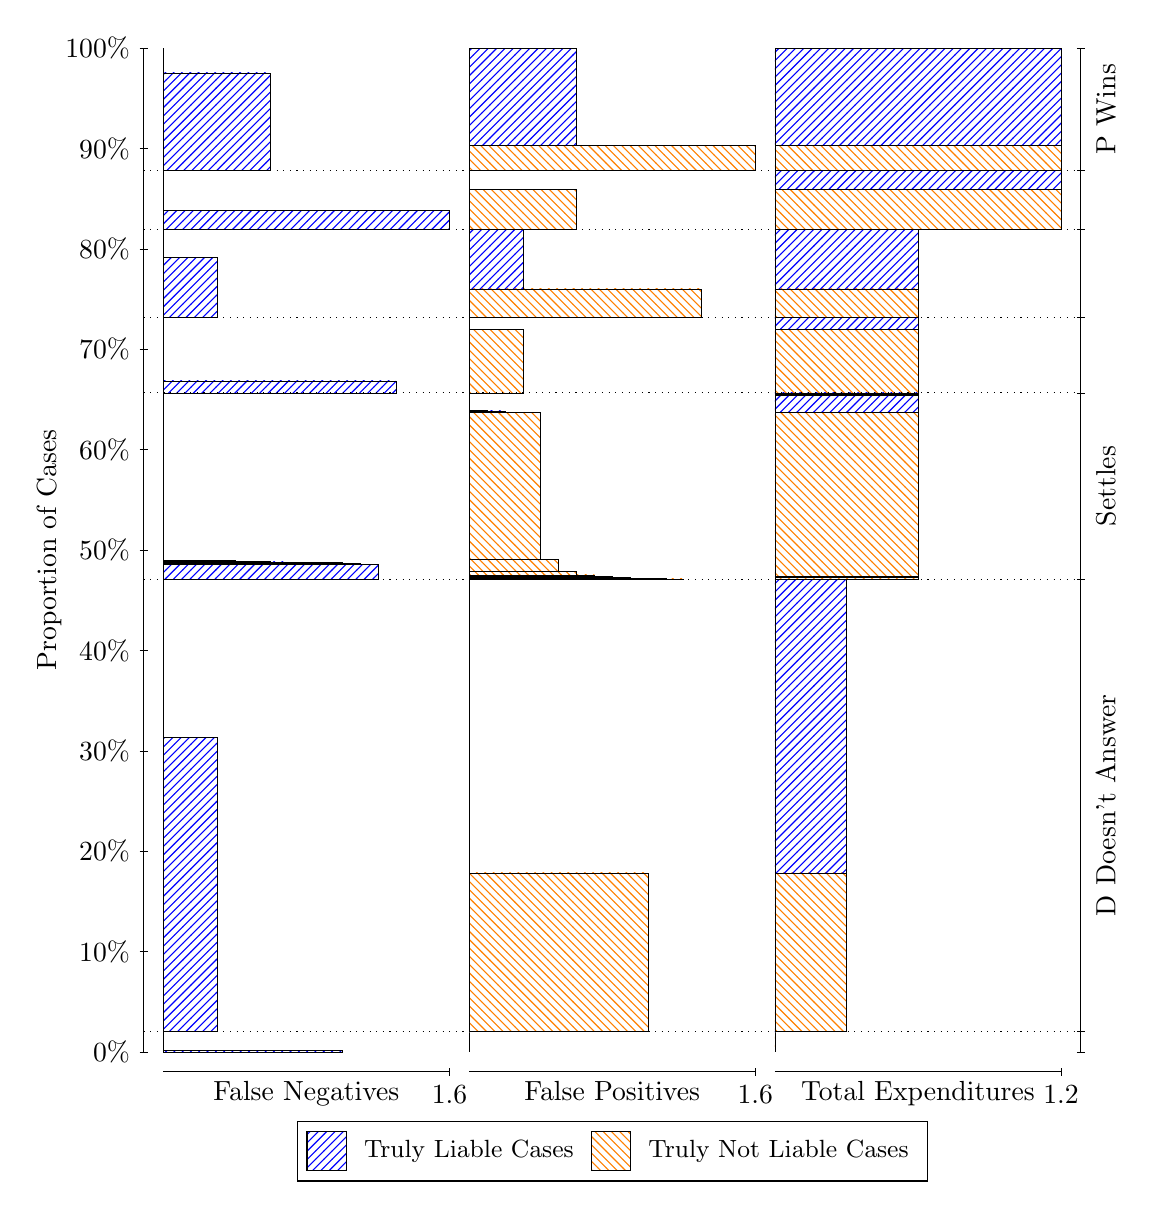
\begin{tikzpicture}
\draw[black, very thin] (1.5,1.75) -- (1.5,14.5);
\node[rotate=90, anchor=center] at (0.3, 8.125) {Proportion of Cases};
\draw[black, very thin] (1.45,1.75) -- (1.55,1.75);
\node[anchor=east] at (1.45, 1.75) {0\%};
\draw[black, very thin] (1.45,3.025) -- (1.55,3.025);
\node[anchor=east] at (1.45, 3.025) {10\%};
\draw[black, very thin] (1.45,4.3) -- (1.55,4.3);
\node[anchor=east] at (1.45, 4.3) {20\%};
\draw[black, very thin] (1.45,5.575) -- (1.55,5.575);
\node[anchor=east] at (1.45, 5.575) {30\%};
\draw[black, very thin] (1.45,6.85) -- (1.55,6.85);
\node[anchor=east] at (1.45, 6.85) {40\%};
\draw[black, very thin] (1.45,8.125) -- (1.55,8.125);
\node[anchor=east] at (1.45, 8.125) {50\%};
\draw[black, very thin] (1.45,9.4) -- (1.55,9.4);
\node[anchor=east] at (1.45, 9.4) {60\%};
\draw[black, very thin] (1.45,10.675) -- (1.55,10.675);
\node[anchor=east] at (1.45, 10.675) {70\%};
\draw[black, very thin] (1.45,11.95) -- (1.55,11.95);
\node[anchor=east] at (1.45, 11.95) {80\%};
\draw[black, very thin] (1.45,13.225) -- (1.55,13.225);
\node[anchor=east] at (1.45, 13.225) {90\%};
\draw[black, very thin] (1.45,14.5) -- (1.55,14.5);
\node[anchor=east] at (1.45, 14.5) {100\%};

\draw[black, very thin] (13.4,1.75) -- (13.4,14.5);
\draw[black, very thin] (13.35,1.75) -- (13.45,1.75);
\node[anchor=west] at (13.35, 1.75) {};
\draw[black, very thin] (13.35,2.0147) -- (13.45,2.0147);
\node[anchor=west] at (13.35, 2.0147) {};
\draw[black, very thin] (13.35,7.7518) -- (13.45,7.7518);
\node[anchor=west] at (13.35, 7.7518) {};
\draw[black, very thin] (13.35,10.121) -- (13.45,10.121);
\node[anchor=west] at (13.35, 10.121) {};
\draw[black, very thin] (13.35,11.079) -- (13.45,11.079);
\node[anchor=west] at (13.35, 11.079) {};
\draw[black, very thin] (13.35,12.201) -- (13.45,12.201);
\node[anchor=west] at (13.35, 12.201) {};
\draw[black, very thin] (13.35,12.945) -- (13.45,12.945);
\node[anchor=west] at (13.35, 12.945) {};
\draw[black, very thin] (13.35,14.5) -- (13.45,14.5);
\node[anchor=west] at (13.35, 14.5) {};

\draw[black, very thin, pattern color=blue, pattern=north east lines] (1.75,1.75) rectangle (4.0208,1.7655);
\draw[black, very thin, pattern color=orange, pattern=north west lines] (1.75,1.7655) rectangle (1.75,2.0147);
\draw[black, very thin, pattern color=blue, pattern=north east lines] (1.75,2.0147) rectangle (2.4312,5.7434);
\draw[black, very thin, pattern color=orange, pattern=north west lines] (1.75,5.7434) rectangle (1.75,7.7518);
\draw[black, very thin, pattern color=blue, pattern=north east lines] (1.75,7.7518) rectangle (4.475,7.9415);
\draw[black, very thin, pattern color=blue, pattern=north east lines] (1.75,7.9415) rectangle (4.2479,7.9568);
\draw[black, very thin, pattern color=blue, pattern=north east lines] (1.75,7.9568) rectangle (4.0208,7.9654);
\draw[black, very thin, pattern color=blue, pattern=north east lines] (1.75,7.9654) rectangle (3.7937,7.9669);
\draw[black, very thin, pattern color=blue, pattern=north east lines] (1.75,7.9669) rectangle (3.7937,7.9677);
\draw[black, very thin, pattern color=blue, pattern=north east lines] (1.75,7.9677) rectangle (3.5667,7.9714);
\draw[black, very thin, pattern color=blue, pattern=north east lines] (1.75,7.9714) rectangle (3.3396,7.9736);
\draw[black, very thin, pattern color=blue, pattern=north east lines] (1.75,7.9736) rectangle (3.1125,7.978);
\draw[black, very thin, pattern color=blue, pattern=north east lines] (1.75,7.978) rectangle (2.8854,7.981);
\draw[black, very thin, pattern color=blue, pattern=north east lines] (1.75,7.981) rectangle (2.6583,7.9964);
\draw[black, very thin, pattern color=orange, pattern=north west lines] (1.75,7.9964) rectangle (1.75,10.121);
\draw[black, very thin, pattern color=blue, pattern=north east lines] (1.75,10.121) rectangle (4.7021,10.273);
\draw[black, very thin, pattern color=orange, pattern=north west lines] (1.75,10.273) rectangle (1.75,11.079);
\draw[black, very thin, pattern color=blue, pattern=north east lines] (1.75,11.079) rectangle (2.4312,11.838);
\draw[black, very thin, pattern color=orange, pattern=north west lines] (1.75,11.838) rectangle (1.75,12.201);
\draw[black, very thin, pattern color=blue, pattern=north east lines] (1.75,12.201) rectangle (5.3833,12.439);
\draw[black, very thin, pattern color=orange, pattern=north west lines] (1.75,12.439) rectangle (1.75,12.945);
\draw[black, very thin, pattern color=blue, pattern=north east lines] (1.75,12.945) rectangle (3.1125,14.183);
\draw[black, very thin, pattern color=orange, pattern=north west lines] (1.75,14.183) rectangle (1.75,14.5);
\draw[black, very thin, pattern color=orange, pattern=north west lines] (5.6333,1.75) rectangle (5.6333,1.9992);
\draw[black, very thin, pattern color=blue, pattern=north east lines] (5.6333,1.9992) rectangle (5.6333,2.0147);
\draw[black, very thin, pattern color=orange, pattern=north west lines] (5.6333,2.0147) rectangle (7.9042,4.0232);
\draw[black, very thin, pattern color=blue, pattern=north east lines] (5.6333,4.0232) rectangle (5.6333,7.7518);
\draw[black, very thin, pattern color=orange, pattern=north west lines] (5.6333,7.7518) rectangle (8.3583,7.7587);
\draw[black, very thin, pattern color=orange, pattern=north west lines] (5.6333,7.7587) rectangle (8.1313,7.7619);
\draw[black, very thin, pattern color=orange, pattern=north west lines] (5.6333,7.7619) rectangle (7.9042,7.7673);
\draw[black, very thin, pattern color=orange, pattern=north west lines] (5.6333,7.7673) rectangle (7.6771,7.7725);
\draw[black, very thin, pattern color=orange, pattern=north west lines] (5.6333,7.7725) rectangle (7.45,7.7916);
\draw[black, very thin, pattern color=orange, pattern=north west lines] (5.6333,7.7916) rectangle (7.2229,7.8084);
\draw[black, very thin, pattern color=orange, pattern=north west lines] (5.6333,7.8084) rectangle (6.9958,7.8536);
\draw[black, very thin, pattern color=orange, pattern=north west lines] (5.6333,7.8536) rectangle (6.7687,8.0073);
\draw[black, very thin, pattern color=orange, pattern=north west lines] (5.6333,8.0073) rectangle (6.5417,9.8767);
\draw[black, very thin, pattern color=blue, pattern=north east lines] (5.6333,9.8767) rectangle (6.0875,9.8922);
\draw[black, very thin, pattern color=blue, pattern=north east lines] (5.6333,9.8922) rectangle (5.8604,9.8952);
\draw[black, very thin, pattern color=blue, pattern=north east lines] (5.6333,9.8952) rectangle (5.6333,10.121);
\draw[black, very thin, pattern color=orange, pattern=north west lines] (5.6333,10.121) rectangle (6.3146,10.927);
\draw[black, very thin, pattern color=blue, pattern=north east lines] (5.6333,10.927) rectangle (5.6333,11.079);
\draw[black, very thin, pattern color=orange, pattern=north west lines] (5.6333,11.079) rectangle (8.5854,11.442);
\draw[black, very thin, pattern color=blue, pattern=north east lines] (5.6333,11.442) rectangle (6.3146,12.201);
\draw[black, very thin, pattern color=orange, pattern=north west lines] (5.6333,12.201) rectangle (6.9958,12.707);
\draw[black, very thin, pattern color=blue, pattern=north east lines] (5.6333,12.707) rectangle (5.6333,12.945);
\draw[black, very thin, pattern color=orange, pattern=north west lines] (5.6333,12.945) rectangle (9.2667,13.262);
\draw[black, very thin, pattern color=blue, pattern=north east lines] (5.6333,13.262) rectangle (6.9958,14.5);
\draw[black, very thin, pattern color=orange, pattern=north west lines] (9.5167,1.75) rectangle (9.5167,1.9992);
\draw[black, very thin, pattern color=blue, pattern=north east lines] (9.5167,1.9992) rectangle (9.5167,2.0147);
\draw[black, very thin, pattern color=orange, pattern=north west lines] (9.5167,2.0147) rectangle (10.425,4.0232);
\draw[black, very thin, pattern color=blue, pattern=north east lines] (9.5167,4.0232) rectangle (10.425,7.7518);
\draw[black, very thin, pattern color=orange, pattern=north west lines] (9.5167,7.7518) rectangle (11.333,7.7795);
\draw[black, very thin, pattern color=blue, pattern=north east lines] (9.5167,7.7795) rectangle (11.333,7.7906);
\draw[black, very thin, pattern color=orange, pattern=north west lines] (9.5167,7.7906) rectangle (11.333,9.8728);
\draw[black, very thin, pattern color=blue, pattern=north east lines] (9.5167,9.8728) rectangle (11.333,10.088);
\draw[black, very thin, pattern color=orange, pattern=north west lines] (9.5167,10.088) rectangle (11.333,10.103);
\draw[black, very thin, pattern color=blue, pattern=north east lines] (9.5167,10.103) rectangle (11.333,10.121);
\draw[black, very thin, pattern color=orange, pattern=north west lines] (9.5167,10.121) rectangle (11.333,10.927);
\draw[black, very thin, pattern color=blue, pattern=north east lines] (9.5167,10.927) rectangle (11.333,11.079);
\draw[black, very thin, pattern color=orange, pattern=north west lines] (9.5167,11.079) rectangle (11.333,11.442);
\draw[black, very thin, pattern color=blue, pattern=north east lines] (9.5167,11.442) rectangle (11.333,12.201);
\draw[black, very thin, pattern color=orange, pattern=north west lines] (9.5167,12.201) rectangle (13.15,12.707);
\draw[black, very thin, pattern color=blue, pattern=north east lines] (9.5167,12.707) rectangle (13.15,12.945);
\draw[black, very thin, pattern color=orange, pattern=north west lines] (9.5167,12.945) rectangle (13.15,13.262);
\draw[black, very thin, pattern color=blue, pattern=north east lines] (9.5167,13.262) rectangle (13.15,14.5);
\draw[black, dotted] (1.5,2.0147) -- (13.4,2.0147);
\draw[black, dotted] (1.5,7.7518) -- (13.4,7.7518);
\draw[black, dotted] (1.5,10.121) -- (13.4,10.121);
\draw[black, dotted] (1.5,11.079) -- (13.4,11.079);
\draw[black, dotted] (1.5,12.201) -- (13.4,12.201);
\draw[black, dotted] (1.5,12.945) -- (13.4,12.945);
\draw[black, very thin] (1.75,1.5) -- (5.3833,1.5);
\node[anchor=north] at (3.5667, 1.5) {False Negatives};
\draw[black, very thin] (5.3833,1.45) -- (5.3833,1.55);
\node[anchor=north] at (5.3833, 1.45) {1.6};

\draw[black, very thin] (5.6333,1.5) -- (9.2667,1.5);
\node[anchor=north] at (7.45, 1.5) {False Positives};
\draw[black, very thin] (9.2667,1.45) -- (9.2667,1.55);
\node[anchor=north] at (9.2667, 1.45) {1.6};

\draw[black, very thin] (9.5167,1.5) -- (13.15,1.5);
\node[anchor=north] at (11.333, 1.5) {Total Expenditures};
\draw[black, very thin] (13.15,1.45) -- (13.15,1.55);
\node[anchor=north] at (13.15, 1.45) {1.2};


\node[black, centered, rotate=90] at (13.72, 4.8833) {D Doesn't Answer};
\node[black, centered, rotate=90] at (13.72, 8.9366) {Settles};



\node[black, centered, rotate=90] at (13.72, 13.722) {P Wins};

\draw (7.449999999999999,1.5) node[draw=none] (baseCoordinate) {};
\begin{scope}[align=center]
        \matrix[scale=0.5, draw=black, below=0.5cm of baseCoordinate, nodes={draw}, column sep=0.1cm]{
            \node[rectangle, draw, minimum width=0.5cm, minimum height=0.5cm, pattern=north east lines, pattern color=blue] {}; &
            \node[draw=none, font=\small] (B) {Truly Liable Cases}; &
            \node[rectangle, draw, minimum width=0.5cm, minimum height=0.5cm, pattern=north west lines, pattern color=orange] {}; &
            \node[draw=none, font=\small] (B) {Truly Not Liable Cases}; \\
            };
\end{scope}

\end{tikzpicture}
\end{document}